\documentclass{article}
\usepackage[paperwidth=275mm,paperheight=135mm,margin=0pt]{geometry}
\usepackage{tikz}
\usepackage{amsmath,amssymb}
\usepackage{xcolor}
\usetikzlibrary{arrows.meta,backgrounds,calc,fit,positioning}
\pagestyle{empty}

\definecolor{panel}{HTML}{FFFFFF}
\definecolor{ink}{HTML}{30343B}
\definecolor{targetgray}{HTML}{777B82}
\definecolor{encoderfill}{HTML}{E8E1F0}
\definecolor{modelfill}{HTML}{F3DCCF}
\definecolor{bodyfill}{HTML}{DDEED6}
\definecolor{latentfill}{HTML}{E4F3FA}
\definecolor{lossfill}{HTML}{FFFFFF}
\definecolor{emphasisred}{HTML}{D94A45}
\definecolor{bluefill}{HTML}{DCEBFA}

\tikzset{
  font=\sffamily\footnotesize,
  >={Latex[length=2.2mm,width=1.4mm]},
  flow/.style={draw=ink, line width=.85pt, ->},
  hotflow/.style={draw=emphasisred, line width=1.05pt, ->},
  target/.style={draw=targetgray, line width=.75pt, dashed, ->},
  box/.style={draw=ink, fill=white, line width=.75pt,
    rounded corners=2pt, align=center, minimum height=9mm,
    inner sep=3pt},
  goalbox/.style={box, fill=bluefill, minimum width=28mm},
  model/.style={box, fill=modelfill, minimum width=23mm},
  encoder/.style={box, fill=encoderfill, minimum width=23mm},
  bodyhead/.style={box, fill=bodyfill, minimum width=25mm},
  latent/.style={box, fill=latentfill, draw=emphasisred, line width=1.1pt,
    minimum width=16mm, font=\sffamily\bfseries\footnotesize},
  scorebox/.style={draw=emphasisred, fill=lossfill, line width=1.25pt,
    rounded corners=3pt, align=center, minimum width=38mm,
    minimum height=11mm, inner sep=3pt},
  lane/.style={draw=ink!28, rounded corners=4pt, line width=.75pt},
  label/.style={font=\sffamily\bfseries\small, text=ink},
  note/.style={fill=panel, inner sep=1pt, font=\scriptsize},
  tag/.style={draw=emphasisred, fill=white, text=emphasisred,
    line width=.9pt, rounded corners=2pt, align=center,
    minimum width=18mm, minimum height=7mm,
    font=\sffamily\bfseries\scriptsize}
}

\begin{document}
\thispagestyle{empty}
\vspace*{\fill}
\noindent\makebox[\paperwidth][c]{%
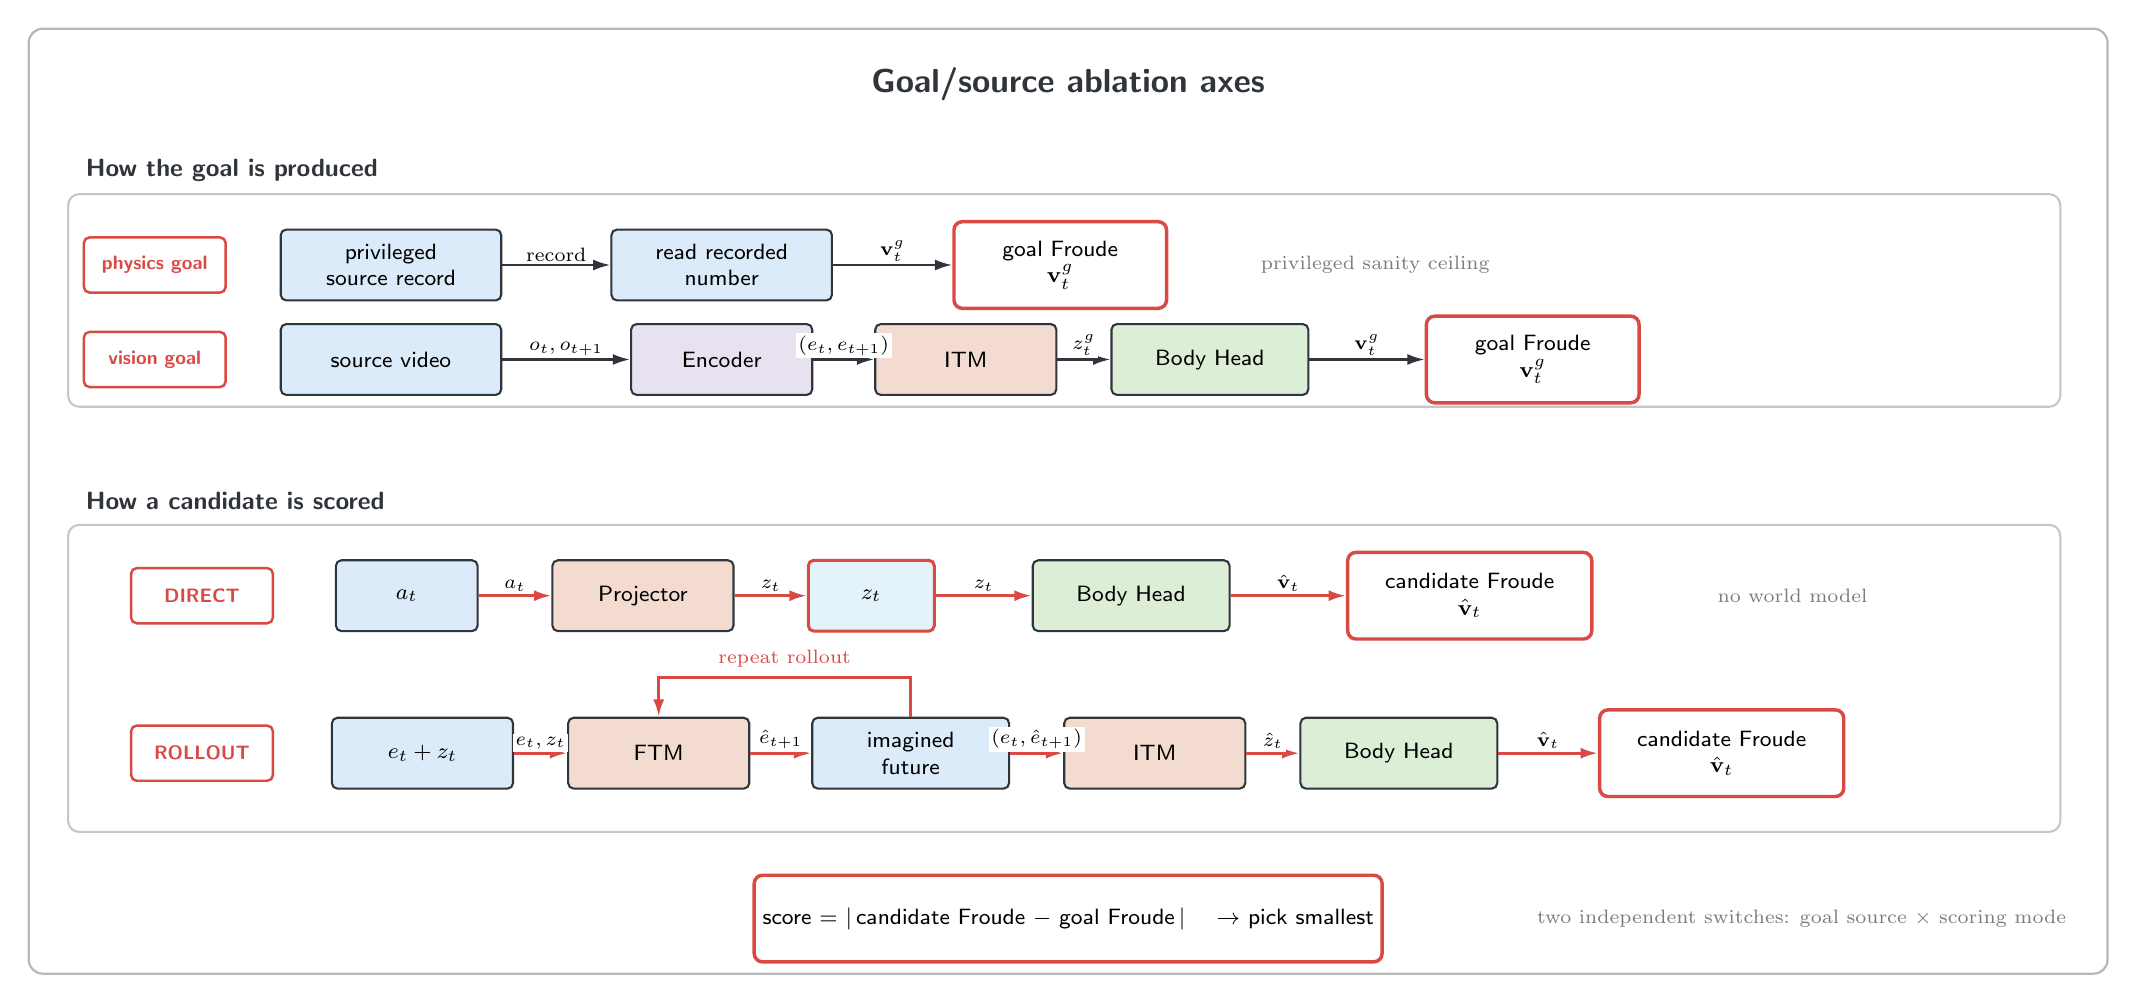
\begin{tikzpicture}[x=1mm,y=1mm]
  \begin{scope}[on background layer]
    \path[draw=ink!35, fill=panel, line width=.8pt, rounded corners=5pt]
      (-8,-60) rectangle (256,60);
  \end{scope}
  \node[font=\sffamily\bfseries\large, text=ink] at (124,53)
    {Goal/source ablation axes};

  % -------------------------------------------------------------------
  % Axis 1: how the goal is produced.
  \node[label, anchor=west] at (-2,42)
    {How the goal is produced};
  \begin{scope}[on background layer]
    \path[lane] (-3,12) rectangle (250,39);
  \end{scope}

  \node[tag] (physicsTag) at (8,30) {physics goal};
  \node[goalbox] (sourceclipA) at (38,30) {privileged\\source record};
  \node[goalbox] (recorded) at (80,30) {read recorded\\number};
  \node[scorebox, minimum width=27mm] (physGoal) at (123,30)
    {goal Froude\\$\mathbf v_t^g$};
  \draw[flow] (sourceclipA) -- node[above,note] {record} (recorded);
  \draw[flow] (recorded) -- node[above,note] {$\mathbf v_t^g$} (physGoal);
  \node[font=\scriptsize, text=targetgray] at (163,30)
    {privileged sanity ceiling};

  \node[tag] (visionTag) at (8,18) {vision goal};
  \node[goalbox] (sourceclipB) at (38,18) {source video};
  \node[encoder] (enc) at (80,18) {Encoder};
  \node[model] (itm) at (111,18) {ITM};
  \node[bodyhead] (bodyheadG) at (142,18) {Body Head};
  \node[scorebox, minimum width=27mm] (visGoal) at (183,18)
    {goal Froude\\$\mathbf v_t^g$};
  \draw[flow] (sourceclipB) -- node[above,note] {$o_t,o_{t+1}$} (enc);
  \draw[flow] (enc) -- node[above,note] {$(e_t,e_{t+1})$} (itm);
  \draw[flow] (itm) -- node[above,note] {$z_t^g$} (bodyheadG);
  \draw[flow] (bodyheadG) -- node[above,note] {$\mathbf v_t^g$} (visGoal);

  % -------------------------------------------------------------------
  % Axis 2: how a candidate is scored.
  \node[label, anchor=west] at (-2,0)
    {How a candidate is scored};
  \begin{scope}[on background layer]
    \path[lane] (-3,-42) rectangle (250,-3);
  \end{scope}

  \node[tag] (directTag) at (14,-12) {DIRECT};
  \node[goalbox, minimum width=18mm] (act) at (40,-12) {$a_t$};
  \node[model] (proj) at (70,-12) {Projector};
  \node[latent] (z) at (99,-12) {$z_t$};
  \node[bodyhead] (bodyheadD) at (132,-12) {Body Head};
  \node[scorebox, minimum width=31mm] (directF) at (175,-12)
    {candidate Froude\\$\hat{\mathbf v}_t$};
  % \draw[hotflow] (directTag) -- (act);
  \draw[hotflow] (act) -- node[above,note] {$a_t$} (proj);
  \draw[hotflow] (proj) -- node[above,note] {$z_t$} (z);
  \draw[hotflow] (z) -- node[above,note] {$z_t$} (bodyheadD);
  \draw[hotflow] (bodyheadD) -- node[above,note] {$\hat{\mathbf v}_t$} (directF);
  \node[font=\scriptsize, text=targetgray] at (216,-12)
    {no world model};

  \node[tag] (rolloutTag) at (14,-32) {ROLLOUT};
  \node[goalbox, minimum width=23mm] (ctx) at (42,-32) {$e_t + z_t$};
  \node[model] (ftm) at (72,-32) {FTM};
  \node[goalbox, minimum width=25mm] (future) at (104,-32) {imagined\\future};
  \node[model] (itmR) at (135,-32) {ITM};
  \node[bodyhead] (bodyheadR) at (166,-32) {Body Head};
  \node[scorebox, minimum width=31mm] (rollF) at (207,-32)
    {candidate Froude\\$\hat{\mathbf v}_t$};
  % \draw[hotflow] (rolloutTag) -- (ctx);
  \draw[hotflow] (ctx) -- node[above,note] {$e_t,z_t$} (ftm);
  \draw[hotflow] (ftm) -- node[above,note] {$\hat e_{t+1}$} (future);
  \draw[hotflow] (future.north) -- ++(0,5) -- ($(ftm.north)+(0,5)$) -- (ftm.north);
  \node[note, text=emphasisred] at (88,-20)
    {repeat rollout};
  \draw[hotflow] (future) -- node[above,note] {$(e_t,\hat e_{t+1})$} (itmR);
  \draw[hotflow] (itmR) -- node[above,note] {$\hat z_t$} (bodyheadR);
  \draw[hotflow] (bodyheadR) -- node[above,note] {$\hat{\mathbf v}_t$} (rollF);

  % -------------------------------------------------------------------
  % Shared decision rule.
  \node[scorebox, minimum width=74mm] at (124,-53)
    {score $=$ $|\,$candidate Froude $-$ goal Froude$\,|$
     \quad $\rightarrow$ pick smallest};

  \node[font=\scriptsize, text=targetgray, anchor=east] at (252,-53)
    {two independent switches: goal source $\times$ scoring mode};
\end{tikzpicture}%
}
\vspace*{\fill}
\end{document}
